\documentclass[11pt]{beamer}

\usetheme{Warsaw}
%\addtobeamertemplate{navigation symbols}{}{%
%    \usebeamerfont{footline}%
%    \usebeamercolor[fg]{footline}%
%    \hspace{1em}%
%    \insertframenumber/\inserttotalframenumber
%}

\beamertemplatenavigationsymbolsempty

\setbeamertemplate{footline}
{
  \leavevmode%
  \hbox{%
  \begin{beamercolorbox}[wd=.333333\paperwidth,ht=2.25ex,dp=1ex,center]{author in head/foot}%
    \usebeamerfont{author in head/foot} \hyperlink{Patrolling Games}{\inserttitle}
  \end{beamercolorbox}%
  \begin{beamercolorbox}[wd=.333333\paperwidth,ht=2.25ex,dp=1ex,center]{title in head/foot}%
    \usebeamerfont{title in head/foot}\insertauthor
  \end{beamercolorbox}%
  \begin{beamercolorbox}[wd=.333333\paperwidth,ht=2.25ex,dp=1ex,right]{date in head/foot}%
    \usebeamerfont{date in head/foot}\insertshortdate{}\hspace*{2em}
    \insertframenumber{} / \inserttotalframenumber\hspace*{2ex} 
  \end{beamercolorbox}}%
  \vskip0pt%
}
\usefonttheme[onlymath]{serif}

\usepackage{color}
\usepackage{xcolor}
\usepackage{tikz}
\usepackage{amsmath}
\usepackage{amssymb}
\usepackage{amsthm}
\usepackage{amsfonts}
\usepackage{graphicx}
\usepackage{mathtools}
\usepackage{wrapfig}
\usepackage{multirow}
\usepackage{comment}
\usepackage{natbib}
\usepackage{appendix}
\usepackage[utf8]{inputenc}
%\usepackage{floatrow}
%\usepackage{newfloat}
\usepackage{subcaption}
\usepackage{bm}
\usepackage{hyperref}

\usetikzlibrary{calc}
\usetikzlibrary{fit}
\usetikzlibrary{shapes.misc,calc, positioning, hobby, backgrounds}


%\DeclarePairedDelimiter{\floor}{\lfloor}{\rightfloor}
%\DeclarePairedDelimiter{\ceil}{\lceil}{\rceil}

\newcommand{\halflength}{\ensuremath{\floor{\frac{m}{2}}}}
\newcommand{\floor}[1]{\left \lfloor #1 \right \rfloor}
\newcommand{\ceil}[1]{\left \lceil #1 \right \rceil}
\newcommand{\pospart}[1]{\left( #1 \right)_{+}}
\newcommand{\negpart}[1]{\left( #1 \right)_{-}}
\newcommand{\set}[2]{\left\{ #1 \, | \, #2 \right\}}

\newcommand{\oneline}[1]{\resizebox{\dimexpr\paperwidth - 3ex}{!}{#1}}

%\DeclareFloatingEnvironment[fileext=los,
 %   listname={List of Example Figures},
  %  name=Example Figure,
   % placement=tbhp,
    %within=section,]{examplefigure}

\author{Thomas Lowbridge}
\title{Patrolling Games}
%\setbeamercovered{transparent} 
%\setbeamertemplate{navigation symbols}{} 
%\logo{} 
\institute{University Of Nottingham} 
\date{December 13, 2017} 
%\subject{} 
\begin{document}

\hypertarget{Patrolling Games}{}
\begin{frame}
\titlepage
\end{frame}

%\begin{frame}
%\tableofcontents
%\end{frame}

\begin{frame}{Outline}

\begin{itemize}
\item Literature review
 \begin{itemize}
 \item Introduction to Game
  \begin{itemize}
  \item \hyperlink{Introduction to Game: Pure Game}{Pure Game}
  \item \hyperlink{Introduction to Game: Mixed Game}{Mixed Game}
  \end{itemize}
 \item Solved Graphs
  \begin{itemize}
  \item \hyperlink{Solved Graphs: Hamiltonian graphs}{Hamiltonian graphs}
  \item \hyperlink{Solved Graphs: Complete bipartite graphs}{Complete bipartite graph}
  \item \hyperlink{Solved Graphs: Star graph}{Star graph}
  \item \hyperlink{Solved Graphs: Line graph}{Line graph}
  \end{itemize}   
 \end{itemize}
\item \hyperlink{Problem with line graph strategy}{Problem with line graph strategy}
\item \hyperlink{Correction of line graph strategy}{Correction of line graph strategy}
\item \hyperlink{Extension of correction strategy}{Extension of correction strategy}
\item \hyperlink{Introduction to the elongated star}{Introduction to the elongated star}
\item \hyperlink{Future work}{Future work}
\end{itemize}
\end{frame}

\hypertarget{Introduction to Game: Pure Game}{}
\begin{frame}{Introduction to Game: Pure Game}

A Patrolling game, $G=G(Q,T,m)$ is made of 3 major components
\begin{itemize}
\item A Graph, $Q=(N,E)$, made of nodes, $N$ ($|N|=n$), and a set of edges, $E$.
\item A time horizon parameter, $T$ (with set $\mathcal{T}=\{0,1,...,T-1\}$).
\item An attack time parameter, $m$.
\end{itemize}

The game involves two players, the patroller and the attacker.
\begin{itemize}
\item The patroller's strategy is a walk (with waiting) on the graph, $W:\mathcal{T} \rightarrow  N$ .
\item The attacker's strategy is a node, $i$ and starting time, $\tau$ .
\end{itemize} 
The strategies are collected into the sets, $\mathcal{W}$ and $\mathcal{A}$ , for the patroller and attacker respectively, with some arbitrary labelling inside the set to form strategies $W_{i}$ and $A_{j}$.

\end{frame}

\begin{frame}{Introduction to Game: Pure Game}
The game is formulated as win-lose (a zero-sum game) with a payoff for the patroller of
\begin{align*}
P(W,(i,\tau))=\left\{ \begin{array}{l}
1 \text{  if  } i \in \left\{ W(\tau),W(\tau+1),...,W(\tau+m-1) \right\} ,\\
0 \text{  if  } i \notin \left\{ W(\tau),W(\tau+1),...,W(\tau+m-1) \right\} .\\
\end{array}\right.
\end{align*}
With a pure payoff matrix $\mathcal{P}=(P(W_{i},A_{j}))_{i \in \{ 1,...,|\mathcal{W}| \}, j \in \{ 1,...,|\mathcal{A}| \}}$
\end{frame}

\begin{frame}{Introduction to Game: Pure Game}
The game played on $Q$ as below with $m=3$ and $T=7$

\begin{center}
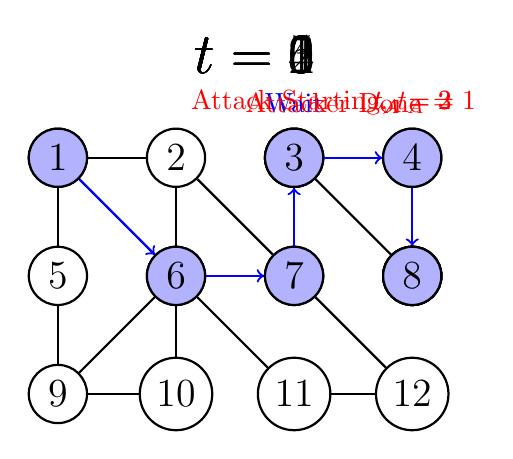
\begin{tikzpicture}[-,auto,node distance=1.5cm,
                    thick,main node/.style={circle,fill=white,draw,font=\sffamily\Large\bfseries}]

  \node[main node] (1) {$1$};
  \node[main node] (2) [right of=1] {$2$};
  \node[main node] (3) [right of=2]  {$3$};
  \node[main node] (4) [right of=3]  {$4$};
  \node[main node] (5) [below of=1]  {$5$};
  \node[main node] (6) [below of=2]  {$6$};
  \node[main node] (7) [below of=3]  {$7$};
  \node[main node] (8) [below of=4]  {$8$};
  \node[main node] (9) [below of=5]  {$9$};
  \node[main node] (10) [below of=6]  {$10$};
  \node[main node] (11) [below of=7] {$11$};
  \node[main node] (12) [below of=8] {$12$}; 

  \path[every node/.style={font=\sffamily}]
    (1) edge (2)
    (1) edge (5)
    (1) edge (6)
    (2) edge (6)
    (2) edge (7)
    (3) edge (7)
    (3) edge (4)
    (3) edge (8)
    (4) edge (8)
    (5) edge (9)
    (6) edge (7)
    (6) edge (10)
    (6) edge (11)
    (6) edge (9)
    (7) edge (12)
    (9) edge (10)
    (11) edge (12)
    ;

 %\node (GraphLabel) [shift={(0,1)}] at (1) {$Q$}; 

%Slide 2 (first animation)
  \visible<2>{
  \node (TimeLabel) [shift={(2.5,1.3)}] at (1) {\huge $t=0$};
  \node[main node,fill=blue!30] (1) at (1) {$1$};
  \path[->,color=blue] (1) edge (6); 
    }
%Slide 3
  \visible<3>{
   \node (TimeLabel) [shift={(2.5,1.3)}] at (1) {\huge $t=1$};
  \node[main node,fill=blue!30] (6) at (6) {$6$};
  \path[->,color=blue] (6) edge (7); 
    }
%Slide 4
  \visible<4>{
   \node (TimeLabel) [shift={(2.5,1.3)}] at (1) {\huge $t=2$};
  \node[main node,fill=blue!30] (7) at (7) {$7$};
  \path[->,color=blue] (7) edge (3);
  
  \node[main node,fill=red!30] (8) at (8) {$8$};
  \node[color=red] (Attacktimelabel) [shift={(-1,2.2)}] at (8) {Attack Starting, $t_{A}=1$};
    }
%Slide 5
  \visible<5>{
   \node (TimeLabel) [shift={(2.5,1.3)}] at (1) {\huge $t=3$};
  \node[main node,fill=blue!30] (3) at (3) {$3$};
  \node[color=blue] (WaitingLabel) [shift={(0,0.7)}] at (3) {Wait};
  
  \node[main node,fill=red!30] (8) at (8) {$8$};
  \node[color=red] (Attacktimelabel) [shift={(0,2.2)}] at (8) {$t_{A}=2$}; 
    }
%Slide 6
  \visible<6>{
   \node (TimeLabel) [shift={(2.5,1.3)}] at (1) {\huge $t=4$};
  \node[main node,fill=blue!30] (3) at (3) {$3$};
  \path[->,color=blue] (3) edge (4);
  
  \node[main node,fill=red!30] (8) at (8) {$8$};  
  \node[color=red] (Attacktimelabel) [shift={(0,2.2)}] at (8) {$t_{A}=3$};
    }
%Slide 7
  \visible<7>{
   \node (TimeLabel) [shift={(2.5,1.3)}] at (1) {\huge $t=5$};
  \node[main node,fill=blue!30] (4) at (4) {$4$};
  \path[->,color=blue] (4) edge (8); 
  
  \node[color=red] (Attacktimelabel) [shift={(-1,2.2)}] at (8) {Attacker Done};
    }    
%Slide 8
  \visible<8>{
   \node (TimeLabel) [shift={(2.5,1.3)}] at (1) {\huge $t=6$};
  \node[main node,fill=blue!30] (8) at (8) {$8$}; 
    }                 
\end{tikzpicture}

\end{center}
\only<1>{
\begin{itemize}
\item[] \textcolor{blue}{Patroller:} \textcolor{blue}{ $W(0)=1$ , $W(1)=6$ , $W(2)= 7$ , $W(3)=3$ , $W(4)=3$ , $W(5)=4$ , $W(8)= 8$}
\item[] \textcolor{red}{Attacker:} \textcolor{red}{$(8,2)$}
\end{itemize}
}
\only<8>
{
The attacker fails to catch the patroller, therefore the patroller loses (and the attacker wins) meaning a payoff of $0$ for the patroller (and $-1$ for the attacker).
}
\end{frame}

\hypertarget{Introduction to Game: Mixed Game}{}
\begin{frame}{Introduction to Game: Mixed Game}
Both the patroller and attacker will play their pure(realised) strategies with certain probabilities, let $\bm{\pi}$ be a mixed strategy for the patroller and let $\bm{\phi}$ be a mixed strategy for the attacker. We collect these into the sets $\Pi$ and $\Phi$ for the patroller and attacker respectively.

Then the payoff for the patroller of this mixed game becomes
\begin{align*}
P(\bm{\pi} ,\bm{\phi})=\sum\limits_{i=1}^{|\mathcal{W}|} \sum\limits_{j=1}^{|\mathcal{I}|} \mathcal{P}_{i,j} \bm{\pi} _{i} \bm{\phi}_{j}
=\bm{\pi} \mathcal{P} \bm{\phi}
\end{align*}

By using the pure payoff as $1$ when capture occurs and $0$ otherwise, the mixed payoff is equivalent to the probability of capture.
\end{frame}

\begin{frame}{Introduction to Game: Mixed Game}
\begin{block}{Mixed Nash equilibrium}
A choice of $\bm{\pi}^*$ and $\bm{\phi}^*$ is said to be in \textit{Nash equilibrium} if 
\begin{align*}
P(\bm{\pi}^*,\bm{\phi}^*) \geq P(\bm{\pi},\bm{\phi}^*) \quad \forall \bm{\pi} \in \Pi , \\
P(\bm{\pi}^*,\bm{\phi}^*) \geq P(\bm{\pi}^*,\bm{\phi}) \quad \forall \bm{\phi} \in \Phi .
\end{align*}
\end{block}
There will only be one Nash equilibrium, unless the patroller can guarantee capture.

We do this by searching for the games value, $$V(G) \equiv \max\limits_{\bm{\pi} \in \Pi} \min\limits_{\bm{\phi} \in \Phi} P(\bm{\pi},\bm{\phi})=\min\limits_{\bm{\phi} \in \Phi} \max\limits_{\bm{\pi} \in \Pi} P(\bm{\pi},\bm{\phi})$$
This is done by achieving both upper and lower bounds on the value of the game.
\end{frame}

\begin{frame}{Solved graphs: Hamiltonian graphs}
\hypertarget{Solved graphs: Hamiltonian graphs}{}

A graph is Hamiltonian if it is possible to find a cycle which visits every node exactly one (apart from the start/finish).

\begin{block}{Hamiltonian graphs}
A Hamiltonian graph has the value $V=\frac{m}{n}$
\end{block}

Two common Hamiltonian graphs are the Cyclic graph (of n nodes $C_{n}$) and the Complete graph (of n nodes $K_{n}$).
\begin{center}
\begin{figure}

\begin{tabular}{@{}c@{}}
  \begin{tabular}{c}
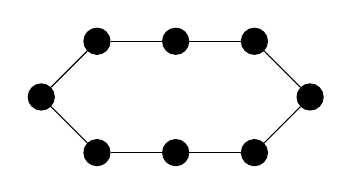
\begin{tikzpicture}[baseline=(current bounding box.north),-,auto,node distance=1cm,
                    main node/.style={circle,draw,fill=black,font=\sffamily\bfseries}]

  \node[main node] (1) {};
  \node[main node] (2) [above right of=1] {};
  \node[main node] (3) [right of=2] {};
  \node[main node] (4) [right of=3] {};
  \node[main node] (5) [below right of=4] {};
  \node[main node] (6) [below left of=5] {};
  \node[main node] (7) [left of=6] {};
  \node[main node] (8) [left of=7] {};
  

  \path[every node/.style={font=\sffamily}]
  (1) edge (2)
  (2) edge (3)
  (3) edge (4)
  (4) edge (5)
  (5) edge (6)
  (6) edge (7)
  (7) edge (8)
  (8) edge (1);

   
\end{tikzpicture}
     
      \\ \small $C_{8}$
  \end{tabular} \qquad
  \begin{tabular}{c}
  
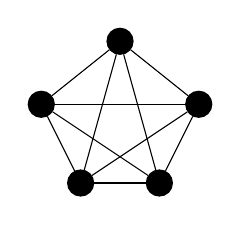
\begin{tikzpicture}[baseline=(current bounding box.north),-,auto,node distance=1cm,
                    main node/.style={circle,draw,fill=black,font=\sffamily\bfseries}]

  \node[main node] (1) {};
  \node[main node] (2) [shift={(1,-0.8)}] at (1) {};
  \node[main node] (3) [shift={(0.5,-1.8)}] at (1) {};
  \node[main node] (4) [shift={(-0.5,-1.8)}] at (1) {};
  \node[main node] (5) [shift={(-1,-0.8)}] at (1) {};

  

  \path[every node/.style={font=\sffamily}]
  (1) edge (2)
      edge (3)
      edge (4)
      edge (5)
  (2) edge (3)
      edge (4)
      edge (5)    
  (3) edge (4)
      edge (5)
  (4) edge (5);


   
\end{tikzpicture}

 \\ \small $K_{5}$
  \end{tabular} \\
\end{tabular}
\caption{Examples of Cyclic and Complete graphs}
\end{figure}
\end{center}



\end{frame}

\hypertarget{Solved graphs: Complete bipartite graphs}{}
\begin{frame}{Solved graphs: Complete bipartite graphs}

A bipartite graph is a graph made of two non-adjacent sets, the complete version has all connections.

\begin{block}{Complete bipartite graph}
A complete bipartite graph, $K_{a,b}$ as value
$V=\frac{m}{2 \max (a,b)}$
\end{block}

\begin{center}
\begin{figure}
\begin{tabular}{c}
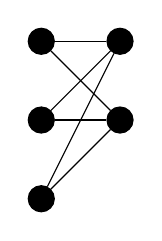
\begin{tikzpicture}[baseline=(current bounding box.north),-,auto,node distance=1cm,
                    main node/.style={circle,draw,fill=black,font=\sffamily\bfseries}]

  \node[main node] (1) {};
  \node[main node] (2) [below of=1] {};
  \node[main node] (3) [below of=2] {};
  \node[main node] (4) [right of=1] {};
  \node[main node] (5) [below of=4] {};

  

  \path[every node/.style={font=\sffamily}]
  (1) edge (4)
      edge (5)
  (2) edge (4)
      edge (5)    
  (3) edge (4)
      edge (5);

   
\end{tikzpicture}
\\ \small $K_{3,2}$
\end{tabular}
\caption{Example of a complete bipartite graph}
\end{figure}

\end{center}

\end{frame}

\hypertarget{Solved graphs: Star graph}{}
\begin{frame}{Solved graphs: Star graph}

The star graph,$S_{n}$, is $n$ nodes adjacent only to the centre. 

\begin{block}{Star graph}
The star $S_{n} \equiv K_{1,n}$ so has the value $V=\frac{m}{2n}$
\end{block}

\begin{center}
\begin{figure}
\begin{tabular}{c}
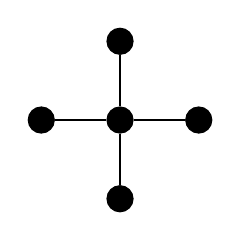
\begin{tikzpicture}[baseline=(current bounding box.north),-,auto,node distance=1cm,
                    main node/.style={circle,draw,fill=black,font=\sffamily\bfseries}]

  \node[main node] (1) {};
  \node[main node] (2) [above of=1] {};
  \node[main node] (3) [right of=1] {};
  \node[main node] (4) [below of=1] {};
  \node[main node] (5) [left of=1] {};

  

  \path[every node/.style={font=\sffamily}]
  (1) edge (2)
      edge (3)
      edge (4)
      edge (5);

   
\end{tikzpicture}
\\ \small $S_{4}$
\end{tabular}
\caption{Example of a star graph}
\end{figure}

\end{center}

\end{frame}

\hypertarget{Solved graphs: Line graph}{}
\begin{frame}{Solved graphs: Line graph}

The line graph, $L_{n}$, made of $n$ nodes each adjacent to two other nodes (apart from the ends)

\begin{block}{Line graph}
The line graph, $L_{n}$ has a value dependent on $(n,m)$
\begin{enumerate}
\item If $m > 2(n-1)$ then $V=1$.
\item If $n-1 < m \leq 2(n-1)$ then $V=\frac{m}{2(n-1)}$
\item If $m=2 , n\geq 3$ then $V=\frac{1}{\ceil{\frac{n}{2}}}$
\item If $m=n-1 \text{ or } m=n-2  \text{ and } m=2k \text{ for some } k \geq 2 $ then $V=\frac{1}{2}$
\item If $3 \leq m \leq n-3$ or  $m=n-2$ and $m=2k+1$ for some  $k \geq 1$ then $V=\frac{m}{m+n-1}$
\end{enumerate}
\end{block}
Note. The solution for $m=1$ is know for every graph as $V=\frac{1}{|N|}=\frac{1}{n}$, and if $m=n=2$ then we know $V=1$.
\end{frame}

\begin{frame}{Solved graphs: Line graph}

\begin{center}
\begin{figure}
\begin{tabular}{c}
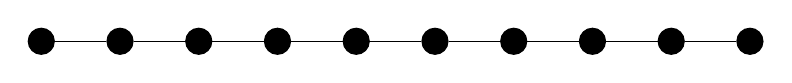
\begin{tikzpicture}[baseline=(current bounding box.north),-,auto,node distance=1cm,
                    main node/.style={circle,draw,fill=black,font=\sffamily\bfseries}]

  \node[main node] (1) {};
  \node[main node] (2) [right of=1] {};
  \node[main node] (3) [right of=2] {};
  \node[main node] (4) [right of=3] {};
  \node[main node] (5) [right of=4] {};
  \node[main node] (6) [right of=5] {};
  \node[main node] (7) [right of=6] {};
  \node[main node] (8) [right of=7] {};
  \node[main node] (9) [right of=8] {};
  \node[main node] (10) [right of=9] {};


  \path[every node/.style={font=\sffamily}]
  (1) edge (2)
  (2) edge (3)
  (3) edge (4)
  (4) edge (5)
  (5) edge (6)
  (6) edge (7)
  (7) edge (8)
  (8) edge (9)
  (9) edge (10);

   
\end{tikzpicture}
\\ \small $L_{10}$
\end{tabular}
\caption{Example of a line graph}
\end{figure}

\end{center}

\begin{columns}[onlytextwidth,T]
   \column{\dimexpr\linewidth-75mm-5mm}
    Regions are:  
    \begin{enumerate}
    \item $m>18$
    \item $9 < m \leq 18$
    \item $m=2$
    \item $m=9,8$
    \item $m=$
    \end{enumerate}

      \column{75mm}
      \begin{minipage}{75mm}
      \begin{figure}
      \resizebox{\linewidth}{!}{
      % Created by tikzDevice version 0.10.1 on 2017-11-09 15:37:15
% !TEX encoding = UTF-8 Unicode
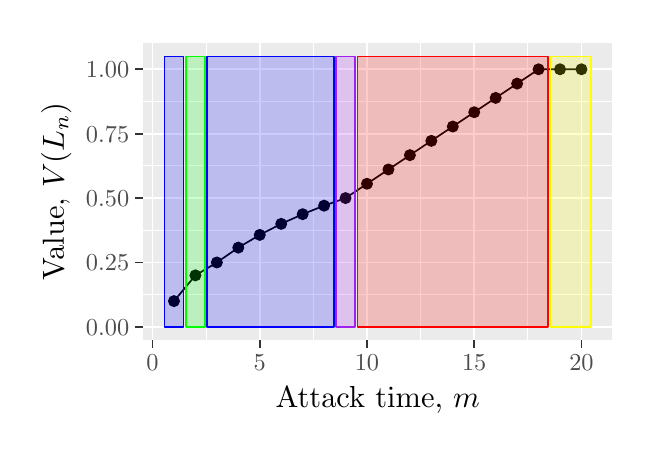
\begin{tikzpicture}[x=1pt,y=1pt]
\definecolor{fillColor}{RGB}{255,255,255}
\path[use as bounding box,fill=fillColor,fill opacity=0.00] (0,0) rectangle (216.81,144.54);
\begin{scope}
\path[clip] (  0.00,  0.00) rectangle (216.81,144.54);
\definecolor{drawColor}{RGB}{255,255,255}
\definecolor{fillColor}{RGB}{255,255,255}

\path[draw=drawColor,line width= 0.6pt,line join=round,line cap=round,fill=fillColor] (  0.00,  0.00) rectangle (216.81,144.54);
\end{scope}
\begin{scope}
\path[clip] ( 41.67, 31.53) rectangle (211.31,139.04);
\definecolor{fillColor}{gray}{0.92}

\path[fill=fillColor] ( 41.67, 31.53) rectangle (211.31,139.04);
\definecolor{drawColor}{RGB}{255,255,255}

\path[draw=drawColor,line width= 0.3pt,line join=round] ( 41.67, 48.05) --
	(211.31, 48.05);

\path[draw=drawColor,line width= 0.3pt,line join=round] ( 41.67, 71.32) --
	(211.31, 71.32);

\path[draw=drawColor,line width= 0.3pt,line join=round] ( 41.67, 94.59) --
	(211.31, 94.59);

\path[draw=drawColor,line width= 0.3pt,line join=round] ( 41.67,117.86) --
	(211.31,117.86);

\path[draw=drawColor,line width= 0.3pt,line join=round] ( 64.49, 31.53) --
	( 64.49,139.04);

\path[draw=drawColor,line width= 0.3pt,line join=round] (103.24, 31.53) --
	(103.24,139.04);

\path[draw=drawColor,line width= 0.3pt,line join=round] (141.99, 31.53) --
	(141.99,139.04);

\path[draw=drawColor,line width= 0.3pt,line join=round] (180.74, 31.53) --
	(180.74,139.04);

\path[draw=drawColor,line width= 0.6pt,line join=round] ( 41.67, 36.42) --
	(211.31, 36.42);

\path[draw=drawColor,line width= 0.6pt,line join=round] ( 41.67, 59.69) --
	(211.31, 59.69);

\path[draw=drawColor,line width= 0.6pt,line join=round] ( 41.67, 82.96) --
	(211.31, 82.96);

\path[draw=drawColor,line width= 0.6pt,line join=round] ( 41.67,106.23) --
	(211.31,106.23);

\path[draw=drawColor,line width= 0.6pt,line join=round] ( 41.67,129.50) --
	(211.31,129.50);

\path[draw=drawColor,line width= 0.6pt,line join=round] ( 45.11, 31.53) --
	( 45.11,139.04);

\path[draw=drawColor,line width= 0.6pt,line join=round] ( 83.86, 31.53) --
	( 83.86,139.04);

\path[draw=drawColor,line width= 0.6pt,line join=round] (122.61, 31.53) --
	(122.61,139.04);

\path[draw=drawColor,line width= 0.6pt,line join=round] (161.36, 31.53) --
	(161.36,139.04);

\path[draw=drawColor,line width= 0.6pt,line join=round] (200.11, 31.53) --
	(200.11,139.04);
\definecolor{drawColor}{RGB}{0,0,0}
\definecolor{fillColor}{RGB}{0,0,0}

\path[draw=drawColor,line width= 0.4pt,line join=round,line cap=round,fill=fillColor] (192.36,129.50) circle (  1.96);

\path[draw=drawColor,line width= 0.4pt,line join=round,line cap=round,fill=fillColor] (200.11,129.50) circle (  1.96);

\path[draw=drawColor,line width= 0.4pt,line join=round,line cap=round,fill=fillColor] (122.61, 88.13) circle (  1.96);

\path[draw=drawColor,line width= 0.4pt,line join=round,line cap=round,fill=fillColor] (130.36, 93.30) circle (  1.96);

\path[draw=drawColor,line width= 0.4pt,line join=round,line cap=round,fill=fillColor] (138.11, 98.47) circle (  1.96);

\path[draw=drawColor,line width= 0.4pt,line join=round,line cap=round,fill=fillColor] (145.86,103.64) circle (  1.96);

\path[draw=drawColor,line width= 0.4pt,line join=round,line cap=round,fill=fillColor] (153.61,108.81) circle (  1.96);

\path[draw=drawColor,line width= 0.4pt,line join=round,line cap=round,fill=fillColor] (161.36,113.99) circle (  1.96);

\path[draw=drawColor,line width= 0.4pt,line join=round,line cap=round,fill=fillColor] (169.11,119.16) circle (  1.96);

\path[draw=drawColor,line width= 0.4pt,line join=round,line cap=round,fill=fillColor] (176.86,124.33) circle (  1.96);

\path[draw=drawColor,line width= 0.4pt,line join=round,line cap=round,fill=fillColor] (184.61,129.50) circle (  1.96);

\path[draw=drawColor,line width= 0.4pt,line join=round,line cap=round,fill=fillColor] ( 60.61, 55.03) circle (  1.96);

\path[draw=drawColor,line width= 0.4pt,line join=round,line cap=round,fill=fillColor] (114.86, 82.96) circle (  1.96);

\path[draw=drawColor,line width= 0.4pt,line join=round,line cap=round,fill=fillColor] (107.11, 80.22) circle (  1.96);

\path[draw=drawColor,line width= 0.4pt,line join=round,line cap=round,fill=fillColor] ( 68.36, 59.69) circle (  1.96);

\path[draw=drawColor,line width= 0.4pt,line join=round,line cap=round,fill=fillColor] ( 76.11, 65.06) circle (  1.96);

\path[draw=drawColor,line width= 0.4pt,line join=round,line cap=round,fill=fillColor] ( 83.86, 69.66) circle (  1.96);

\path[draw=drawColor,line width= 0.4pt,line join=round,line cap=round,fill=fillColor] ( 91.61, 73.65) circle (  1.96);

\path[draw=drawColor,line width= 0.4pt,line join=round,line cap=round,fill=fillColor] ( 99.36, 77.14) circle (  1.96);

\path[draw=drawColor,line width= 0.4pt,line join=round,line cap=round,fill=fillColor] ( 52.86, 45.73) circle (  1.96);

\path[draw=drawColor,line width= 0.6pt,line join=round] ( 52.86, 45.73) --
	( 60.61, 55.03) --
	( 68.36, 59.69) --
	( 76.11, 65.06) --
	( 83.86, 69.66) --
	( 91.61, 73.65) --
	( 99.36, 77.14) --
	(107.11, 80.22) --
	(114.86, 82.96) --
	(122.61, 88.13) --
	(130.36, 93.30) --
	(138.11, 98.47) --
	(145.86,103.64) --
	(153.61,108.81) --
	(161.36,113.99) --
	(169.11,119.16) --
	(176.86,124.33) --
	(184.61,129.50) --
	(192.36,129.50) --
	(200.11,129.50);
\definecolor{drawColor}{RGB}{255,255,0}
\definecolor{fillColor}{RGB}{255,255,0}

\path[draw=drawColor,line width= 0.6pt,line join=round,fill=fillColor,fill opacity=0.20] (188.87, 36.42) rectangle (203.60,134.15);
\definecolor{drawColor}{RGB}{255,0,0}
\definecolor{fillColor}{RGB}{255,0,0}

\path[draw=drawColor,line width= 0.6pt,line join=round,fill=fillColor,fill opacity=0.20] (119.13, 36.42) rectangle (188.10,134.15);
\definecolor{drawColor}{RGB}{160,32,240}
\definecolor{fillColor}{RGB}{160,32,240}

\path[draw=drawColor,line width= 0.6pt,line join=round,fill=fillColor,fill opacity=0.20] (111.38, 36.42) rectangle (118.35,134.15);
\definecolor{drawColor}{RGB}{0,0,255}
\definecolor{fillColor}{RGB}{0,0,255}

\path[draw=drawColor,line width= 0.6pt,line join=round,fill=fillColor,fill opacity=0.20] ( 64.88, 36.42) rectangle (110.60,134.15);
\definecolor{drawColor}{RGB}{0,255,0}
\definecolor{fillColor}{RGB}{0,255,0}

\path[draw=drawColor,line width= 0.6pt,line join=round,fill=fillColor,fill opacity=0.20] ( 57.13, 36.42) rectangle ( 64.10,134.15);
\definecolor{drawColor}{RGB}{0,0,255}
\definecolor{fillColor}{RGB}{0,0,255}

\path[draw=drawColor,line width= 0.6pt,line join=round,fill=fillColor,fill opacity=0.20] ( 49.38, 36.42) rectangle ( 56.35,134.15);
\end{scope}
\begin{scope}
\path[clip] (  0.00,  0.00) rectangle (216.81,144.54);
\definecolor{drawColor}{gray}{0.30}

\node[text=drawColor,anchor=base east,inner sep=0pt, outer sep=0pt, scale=  0.88] at ( 36.72, 33.39) {0.00};

\node[text=drawColor,anchor=base east,inner sep=0pt, outer sep=0pt, scale=  0.88] at ( 36.72, 56.66) {0.25};

\node[text=drawColor,anchor=base east,inner sep=0pt, outer sep=0pt, scale=  0.88] at ( 36.72, 79.93) {0.50};

\node[text=drawColor,anchor=base east,inner sep=0pt, outer sep=0pt, scale=  0.88] at ( 36.72,103.20) {0.75};

\node[text=drawColor,anchor=base east,inner sep=0pt, outer sep=0pt, scale=  0.88] at ( 36.72,126.47) {1.00};
\end{scope}
\begin{scope}
\path[clip] (  0.00,  0.00) rectangle (216.81,144.54);
\definecolor{drawColor}{gray}{0.20}

\path[draw=drawColor,line width= 0.6pt,line join=round] ( 38.92, 36.42) --
	( 41.67, 36.42);

\path[draw=drawColor,line width= 0.6pt,line join=round] ( 38.92, 59.69) --
	( 41.67, 59.69);

\path[draw=drawColor,line width= 0.6pt,line join=round] ( 38.92, 82.96) --
	( 41.67, 82.96);

\path[draw=drawColor,line width= 0.6pt,line join=round] ( 38.92,106.23) --
	( 41.67,106.23);

\path[draw=drawColor,line width= 0.6pt,line join=round] ( 38.92,129.50) --
	( 41.67,129.50);
\end{scope}
\begin{scope}
\path[clip] (  0.00,  0.00) rectangle (216.81,144.54);
\definecolor{drawColor}{gray}{0.20}

\path[draw=drawColor,line width= 0.6pt,line join=round] ( 45.11, 28.78) --
	( 45.11, 31.53);

\path[draw=drawColor,line width= 0.6pt,line join=round] ( 83.86, 28.78) --
	( 83.86, 31.53);

\path[draw=drawColor,line width= 0.6pt,line join=round] (122.61, 28.78) --
	(122.61, 31.53);

\path[draw=drawColor,line width= 0.6pt,line join=round] (161.36, 28.78) --
	(161.36, 31.53);

\path[draw=drawColor,line width= 0.6pt,line join=round] (200.11, 28.78) --
	(200.11, 31.53);
\end{scope}
\begin{scope}
\path[clip] (  0.00,  0.00) rectangle (216.81,144.54);
\definecolor{drawColor}{gray}{0.30}

\node[text=drawColor,anchor=base,inner sep=0pt, outer sep=0pt, scale=  0.88] at ( 45.11, 20.52) {0};

\node[text=drawColor,anchor=base,inner sep=0pt, outer sep=0pt, scale=  0.88] at ( 83.86, 20.52) {5};

\node[text=drawColor,anchor=base,inner sep=0pt, outer sep=0pt, scale=  0.88] at (122.61, 20.52) {10};

\node[text=drawColor,anchor=base,inner sep=0pt, outer sep=0pt, scale=  0.88] at (161.36, 20.52) {15};

\node[text=drawColor,anchor=base,inner sep=0pt, outer sep=0pt, scale=  0.88] at (200.11, 20.52) {20};
\end{scope}
\begin{scope}
\path[clip] (  0.00,  0.00) rectangle (216.81,144.54);
\definecolor{drawColor}{RGB}{0,0,0}

\node[text=drawColor,anchor=base,inner sep=0pt, outer sep=0pt, scale=  1.10] at (126.49,  7.44) {Attack time, $m$};
\end{scope}
\begin{scope}
\path[clip] (  0.00,  0.00) rectangle (216.81,144.54);
\definecolor{drawColor}{RGB}{0,0,0}

\node[text=drawColor,rotate= 90.00,anchor=base,inner sep=0pt, outer sep=0pt, scale=  1.10] at ( 13.08, 85.29) {Value, $V(L_{n})$};
\end{scope}
\end{tikzpicture}
}
      \caption{Value of the line graph for varying $m$}
      \end{figure}
      \end{minipage}


    \end{columns}


\end{frame}


\hypertarget{Problem with line graph strategy}{}
\begin{frame}{Problem with line graph strategy}

It was initially stated that in the region two $n-1 \leq m \leq 2(n-1)$, the value $\frac{m}{2(n-1)}$ is achieved by the attacker attacking using the \textcolor{red}{diametric strategy}, which is to attack at opposite ends of the line with equal probability for all possible starting times. This is supposed to guarantee that $V \leq \frac{m}{2(n-1)}$.
\newline
\newline
\textbf{Example.}
Consider $L_{5}$ with $T=m=5$ , then the patroller only needs to walk between the end nodes to win.
\begin{center}
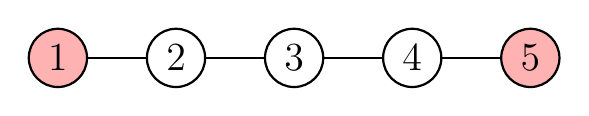
\begin{tikzpicture}[-,auto,node distance=1.5cm,
                    thick,main node/.style={circle,fill=white,draw,font=\sffamily\Large\bfseries}]

  \node[main node,fill=red!30] (1) {$1$};
  \node[main node] (2) [right of=1] {$2$};
  \node[main node] (3) [right of=2]  {$3$};
  \node[main node] (4) [right of=3]  {$4$};
  \node[main node,fill=red!30] (5) [right of=4] {$5$};

  \path[every node/.style={font=\sffamily}]
    (1) edge (2)
    (2) edge (3)
    (3) edge (4)
    (4) edge (5)
    ;
\end{tikzpicture}
\end{center}
The walk $\{ 1,2,3,4,5 \}$ guarantee's the capture of all attacks made.

\end{frame}

\begin{frame}{Problem with line graph strategy}

\textbf{Example.}
Consider $L_{31}$ with $m=45$

\begin{figure}
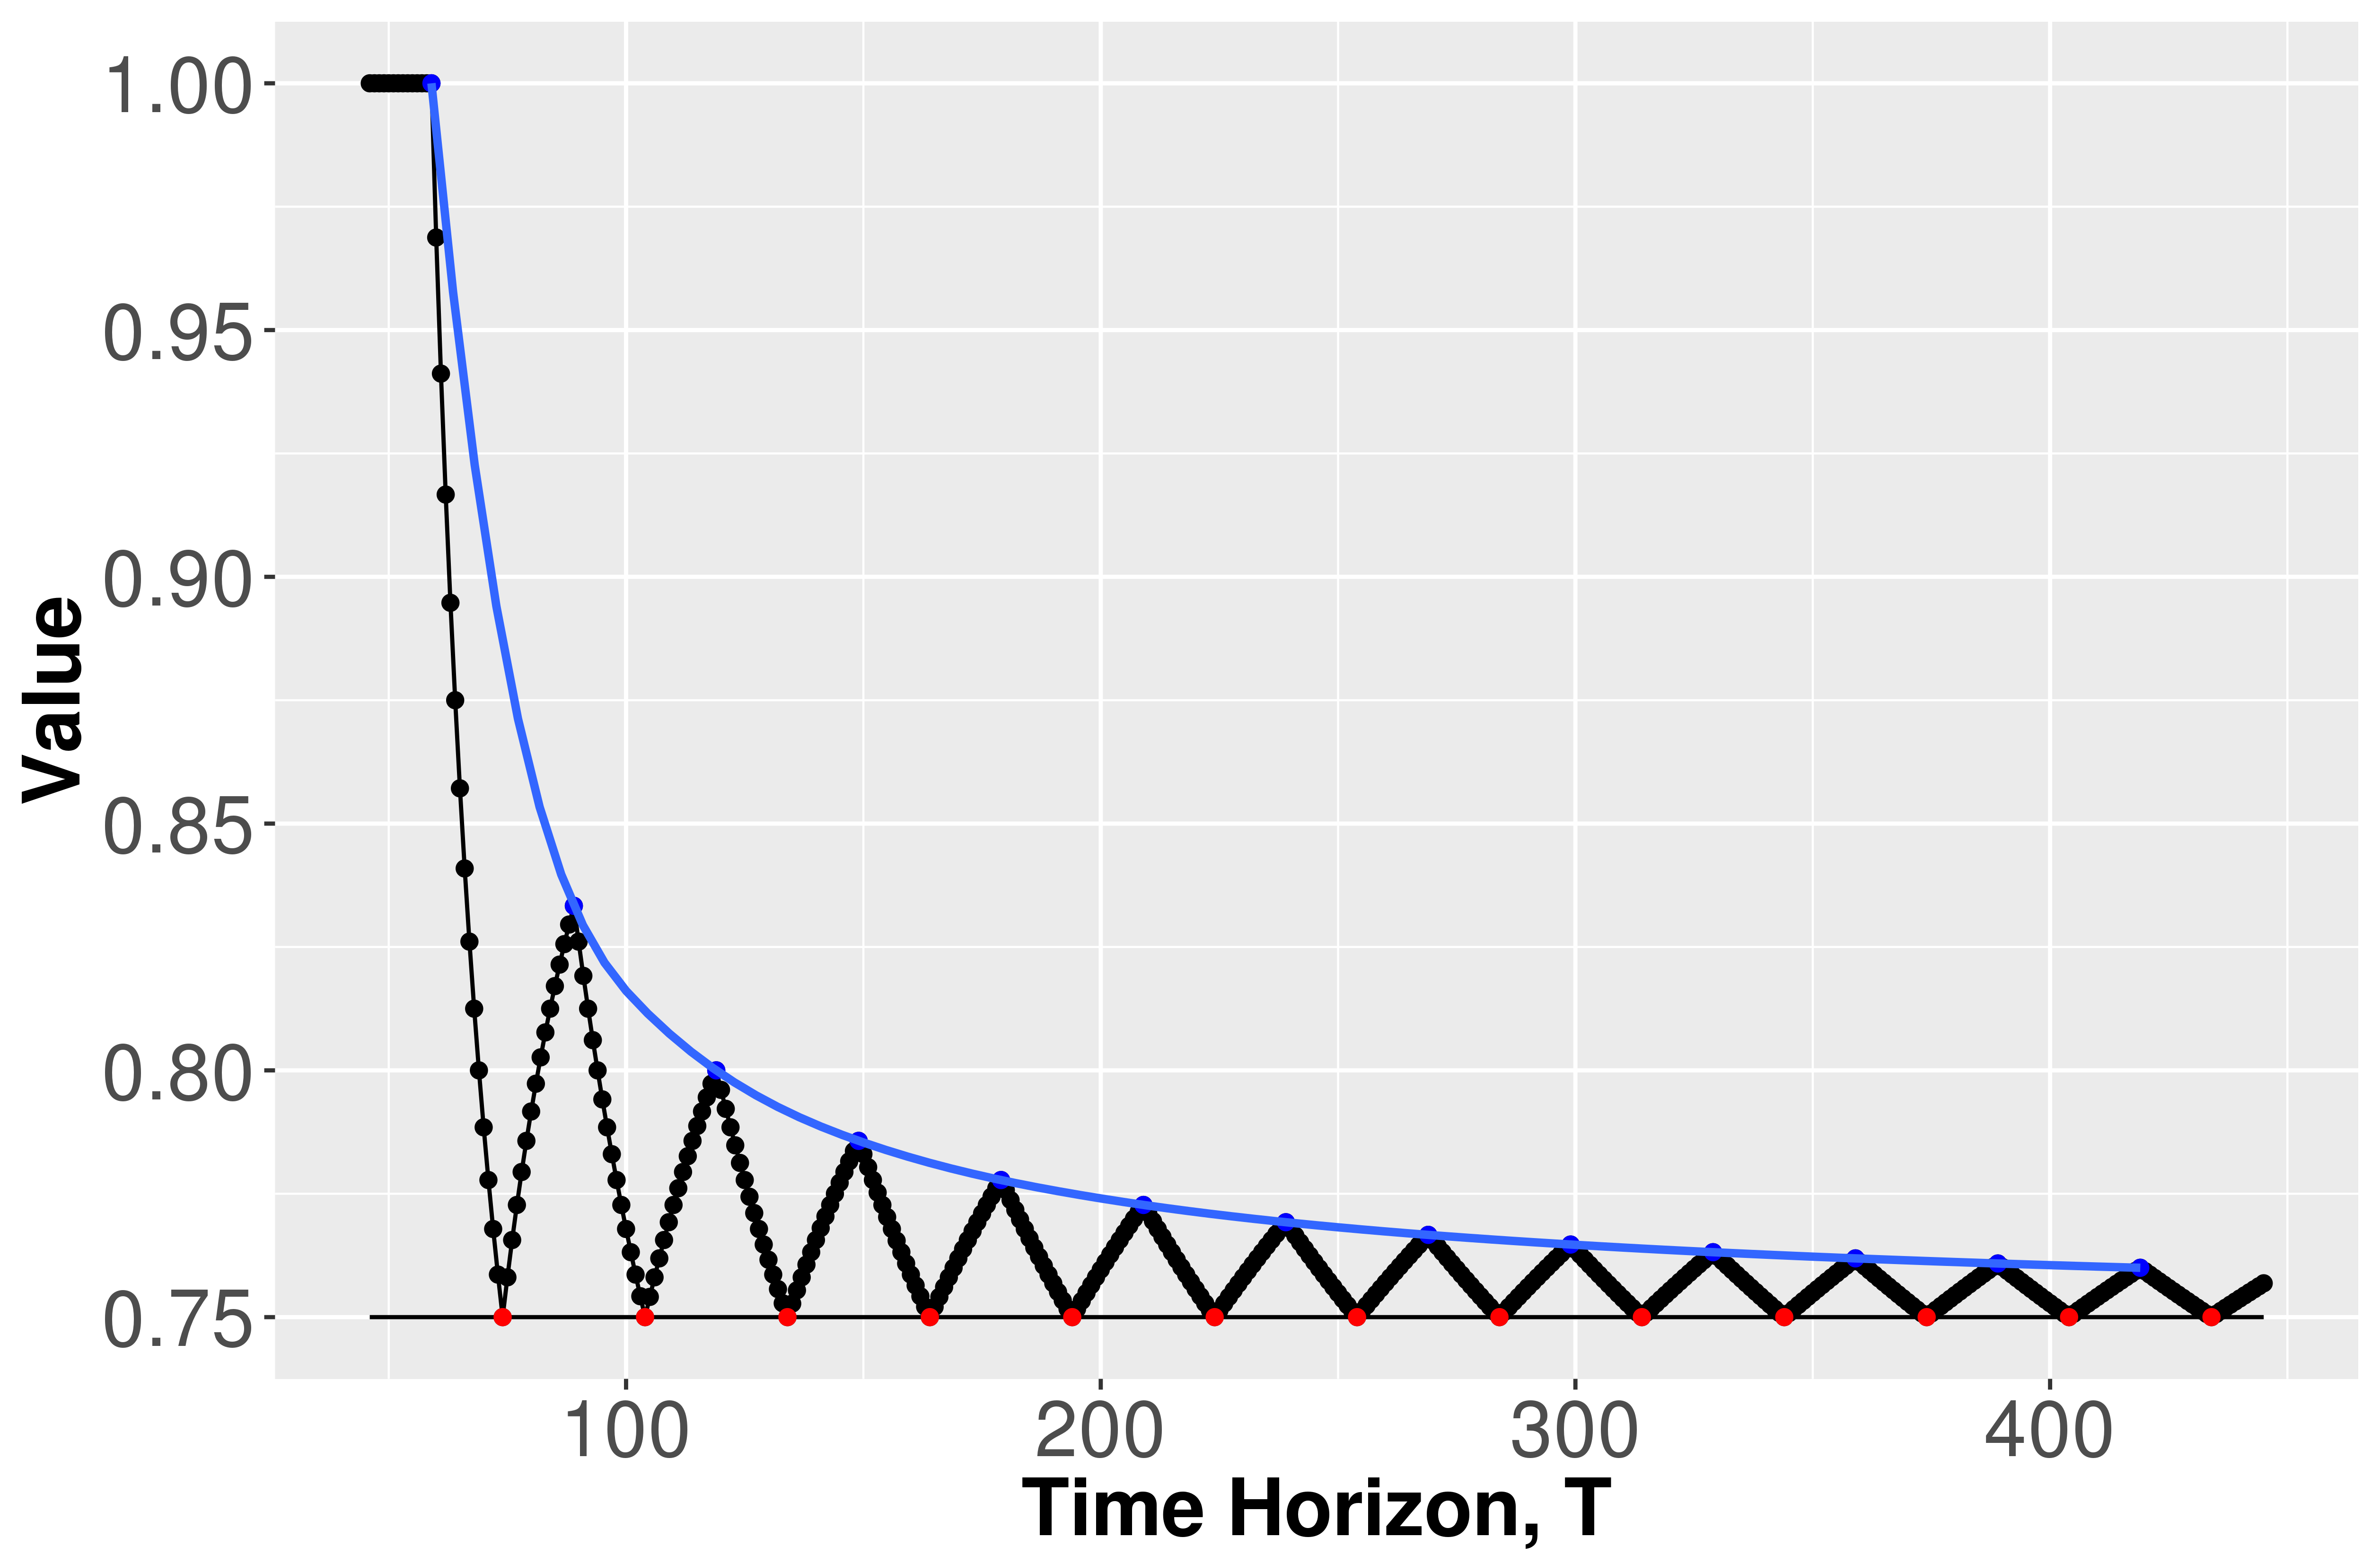
\includegraphics[scale=0.4]{DiametricAttack(m_45,d_30)1.png}
\caption{Best Upper Bound achievable under the diametric strategy}
\end{figure}

\end{frame}

\begin{frame}{Problem with the line graph strategy}

The problem is under the diametric attack, a patroller can catch
\tiny

\begin{align*}
&m-\bar{d}+\pospart{m \times (\floor{\frac{T-2m+1}{\bar{d}}}+1)} +  \pospart{T-(m-1+(\floor{\frac{T-2m+1}{\bar{d}}}+1)\bar{d})} +  \\
&\hspace{75pt} \pospart{T-(m-1+(\floor{\frac{T-2m+1}{\bar{d}}}+2)\bar{d})}
\end{align*}

\normalsize
attacks. From this we can get

\begin{lemma}[Condition on $T$ for bound to hold]
When $T=m-1+(k+1)(n-1)$ for some $k \in \mathbb{N}_{0}$ then the diametric bound holds. Otherwise as $T \rightarrow \infty$ then the diametric bound, $V \leq \frac{m}{2(n-1)}$, holds.
\end{lemma}

\end{frame}

\hypertarget{Correction to Line graph strategy}{}
\begin{frame}{Correction of line graph strategy}
We propose a solution to the problem, by limiting the time

\begin{definition}[Time limited diametric attack]
When $T \geq m+n-2$ we have the \textit{time limited diametric attack} (on the line) strategy is for the attacker to attack at both ends of the line with equal probability for starting times $0,1,...,n-2$
\end{definition}

This restriction to the attacking time guarantees to get the upper bound of $V \leq \frac{m}{2(n-1)}$. 

This works due to the spacing of the attack times.
\end{frame}

\hypertarget{Extension of correction strategy}{}
\begin{frame}{Extension of correction strategy}


Let $\bar{d}$ be the diameter of the graph, i.e the distance between the furthest apart nodes then using

\begin{definition}[Time limited diametric attack]
When $T \geq m-1+\bar{d}$ we have the \textit{time limited diametric attack} strategy is for the attacker to attack at both ends of the line with equal probability for starting times $\tau,\tau +1,...,\tau + \bar{d}-1$ (for a chosen initial $\tau$).
\end{definition}

\begin{lemma}[Time limited diametric bound]
When $T \geq m-1 +\bar{d}$ the attacker can get the bound
$$V \leq \dfrac{m}{2\bar{d}}.$$
\end{lemma}

\end{frame}


\begin{frame}{Extension of correction strategy}
Using $d(i,j)$ as the distance between nodes $i$ and $j$ we can get a more general type of attack.

\begin{definition}[Polygonal attack]
A \textit{$d$-polygonal attack} is an attack at a set of nodes $D= \set{i \in N}{ d(i,j)=d , \forall j \in D}$ at the time intervals $\tau,\tau+1,...,\tau+d-1$ (for a chosen initial $\tau$) all equally probable.
\end{definition}

\begin{lemma}[Polygonal bound]
When $T \geq m+d-1$ and a set $D$ as in the $d$-polygonal attack exists, the value has an upper bound of $V \leq \max \{ \frac{1}{|D|} , \frac{m}{|D|d} \}$ .
\end{lemma}

\end{frame}

\hypertarget{Introduction to the elongated star}{}
\begin{frame}{Introduction to the elongated star}


We now wish to integrate features of a star into a line.
We will form the elongated star $S_{n}^{k}$. We will use the labelling as below

\begin{figure}
\begin{center}
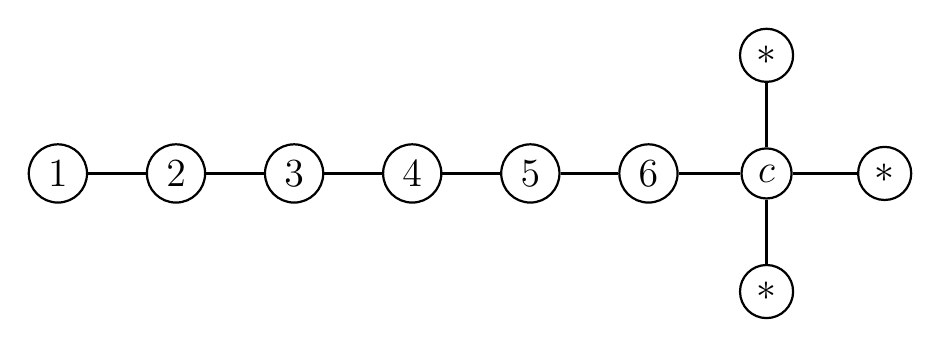
\begin{tikzpicture}[-,auto,node distance=1.5cm,
                    thick,main node/.style={circle,draw,font=\sffamily\Large\bfseries}]

  \node[main node] (1) {$1$};
  \node[main node] (2) [right of=1] {$2$};
  \node[main node] (3) [right of=2] {$3$};
  \node[main node] (4) [right of=3] {$4$};
  \node[main node] (5) [right of=4] {$5$};
  \node[main node] (6) [right of=5]  {$6$};
  \node[main node] (7) [right of=6]  {$c$};
  \node[main node] (8) [right of=7]  {$*$};
  \node[main node] (9) [above of=7]  {$*$};
  \node[main node] (10) [below of=7]  {$*$};
  

  \path[every node/.style={font=\sffamily}]
    (1) edge  (2)
    (2) edge (3)
    (3) edge (4)
    (4) edge (5)
    (5) edge (6)
    (6) edge (7)
    (7) edge (8)
     edge (9)
     edge (10);
\end{tikzpicture}
\end{center}
\caption{Labeling on the graph $S_{4}^5$.}
\end{figure}

\end{frame}

\hypertarget{Future work}{}
\begin{frame}{Future work}
\end{frame}

\end{document}